\documentclass{article}
\usepackage{multirow}
\usepackage{ifpdf}
\usepackage{graphicx}
\usepackage[colorlinks,bookmarksopen,linkcolor=black,pdfauthor={x},urlcolor=blue]{hyperref}
\usepackage[colorlinks,bookmarksopen]{hyperref}
\usepackage{lgrind}
\usepackage[lined,ruled,linesnumbered,commentsnumbered] {algorithm2e}

\begin{document}
\begin{center}
\textbf{SRI JAYACHAMARAJENDRA COLLEGE OF ENGINEERING}
\textbf{MYSORE-570006}\\
\textsc{department of computer science and engineering}\\
\end{center}

\thispagestyle{empty}
\begin{figure}[htb]
\begin{center}
\ifpdf

\includegraphics[scale=0.30]{logo.png}
\else
%	\includegraphics[scale=0.30]{college logo}
\fi
\end{center}
\end{figure}

\begin{center}
\textbf{MINESWEEPER and LENGTH CONQUER\\}
\end{center}
\begin{center}
\textbf{Submitted by}\\



\begin{tabular}{|c|c|c|}
\hline
Name&Roll No.&Usn\\
\hline
Jayavant M Nijagal&61&4JC09CS126\\
\hline
Nandini Bhavasar N. A &29&4JC09CS060\\
\hline
Sachin Pandit& 45 &4JC09CS090\\
\hline
Vinay.V.Vasista &58&4JC09CS120\\
\hline
\end{tabular}
\end{center}
\vspace*{1cm}
\begin{center}
\emph{\\Guidance of}\\
\textbf{P.M.SHIVAMURTHY}\\
\textit{Lecturer}\\
\textit{Dept of CS$\&$E,SJCE Mysore.}\\
\begin{figure}[htb]
\begin{center}
\ifpdf

\includegraphics[scale=0.30]{vtu.png}
\else
%       \includegraphics[scale=0.30]{college logo}
\fi
\end{center}
\end{figure}
\textbf{Affiliated to}\\
\textbf{VISVESVARAYA TECHNOLOGICAL UNIVERSITY}\\
\textbf{BELGAUM}
\end{center}

\newpage
\tableofcontents




\newpage
\section {Introduction}
\subsection{Minesweeper}
Minesweeper is a single-player game. The object of the game is to clear an abstract minefield without detonating a mine. The game has been written for many system platforms in use today, including the Minesweeper for the Windows platform, which has come bundled with versions of the operating system from 3.1 and on.\\
Minesweeper cannot always be solved with 100 percent certainty, and may require the occasional use of probability to flag the square most likely to have a mine. In other words, one must sometimes guess to solve a minesweeper puzzle.\\
The player is initially presented with a grid of undistinguished squares. Some randomly selected squares, unknown to the player, are designated to contain mines. Typically, the size of the grid and the number of mines are set in advance by the user, either by entering the numbers or selecting from defined skill levels depending on the implementation.\\
The game is played by revealing squares of the grid, typically by clicking them with a mouse. If a square containing a mine is revealed, the player loses the game. Otherwise, a digit is revealed in the square, indicating the number of adjacent squares (typically, out of the possible eight) that contain mines. In typical implementations, if this number is zero then the square appears blank, and the surrounding squares are automatically also revealed. By using logic, the player can in many instances use this information to deduce that certain other squares are mine-free, in which case they may be safely revealed, or mine-filled, in which they can be marked as such (which, in typical implementations, is effected by right-clicking the square and indicated by a flag graphic).\\
The game is won when all mine-free squares are revealed, meaning that all mines have been located.\\
There are many patterns of numbered squares that may arise during a game that can be recognized as allowing only one possible configuration of mines in their vicinity. In the interest of finishing quickly, it is often easiest to process the known patterns first, and continue on with the uncertain parts later. There are a few broad methods for solving problems in minesweeper games without guessing.\\
There are two special cases that are of extra interest when solving a board that can be solved using analysis of only one square and its surrounding squares\\
    $*$ If the number of unrevealed (blank or flagged) squares adjacent to a numbered square is equal to the number on that square, all these unrevealed squares must be mines.
    $*$ For any numbered square, if the number of flagged mines located adjacent to that square is equal to the number of the square, all other squares adjacent to that numbered square must be 'safe'\\

The objective of this project is to implement this game and to make it more interesting as well as more challenging to the player.\\

\newpage
\subsection{Length Conquer }
Length Conquer is a game played by 2 players. The goal of the game is to cover a total length in a scale. To achieve the goal three small sub-units are used. Each player is given a chance alternatively to choose a sub-unit. If the whole scale is covered exactly then the game is a draw. Else the player who last bid will be the winner\\

The objective of this project is to implement this game with one of the player being the computer. The aim is to make the computer unbeatable. This is achieved by designing an algorithm which tells the computer as to which is the safest next move based on all the probable moves of the other player. Care is taken such that the computer always stays in the safer zone. The game will either end up in a draw or the computer will win. \\



\newpage 
\section{Design of algorithm}
\subsection{Minesweeper}
\begin{algorithm}
 \SetKwInOut{Input}{input}
 \SetKwInOut{Output}{output}
 \dontprintsemicolon
\Input{ The choice of user ( easy ==1, medium = 2, hard = 3)}
\Output{Number of mines} 
\Begin{

	if mines $==$ 1
		\\return 13 
	\\else mines $==$ 2
		\\return 28 
	\\else mines $==$ 3
		\\return 40 
	\\else
		return 0 
}
  \caption {Takes the difficulty level from the user }
 \end{algorithm}
 
 
 \begin{algorithm}
 \SetKwInOut{Input}{input}
 \SetKwInOut{Output}{output}
 \dontprintsemicolon
\Input{The position of current cell}
\Output{Number of mines surrounding it} 
\Begin{
count $\leftarrow$ 0 
	\\for i $\leftarrow$ m$-$1 to m$+$1 do
		\\for j $\leftarrow$ n$-$1 to n$+$1 do
			\\if (i $!=$ m OR j $!=$ n) AND (board[i][j] $=$ '$*$')
				\\count $\leftarrow$ count $+$ 1 
	num[m][n] $\leftarrow$ count$+$'0' 

}
  \caption { Procedure to set the values to each cell depending upon the surrounding mines}
 \end{algorithm}

\begin{algorithm}
 \SetKwInOut{Input}{input}
 \SetKwInOut{Output}{output}
 \dontprintsemicolon
\Input{ position of row and column}
\Output{Assigns the value to each cell} 
\Begin{
    countmines $\leftarrow$ 0
	\\nomines $\leftarrow$ numofmines(mines)  		
	\\while nomines $!=$ 0 do
		\\i $\leftarrow$ random number, 0$-$9				
	 	\\j $\leftarrow$ random number, 0$-$9 
		\\if( i $>$ 0 AND i $<$ 9) AND (j $>$ 0 AND j $<$ 9 ) AND board[i$+$1][j$+$1] $!=$ '$*$' 
			\\board[i$+$1][j$+$1] <- '$*$' 
			\\countmines $\leftarrow$ countmines $+$ 1 
		\\nomines $\leftarrow$ nomines $-$ 1
	    \\countmines $\leftarrow$ countmines $-$ 1
	    \\return countmines

}
  \caption { Depending on the difficulty level chosen by the user number of mines are decided}
 \end{algorithm}
 

 \begin{algorithm}
 \SetKwInOut{Input}{input}
 \SetKwInOut{Output}{output}
 \dontprintsemicolon
\Input{}
\Output{} 
\Begin{for i $\leftarrow$ x$-$1 to x$+$1 do
	     \\for j $\leftarrow$ x$-$1 to x$+$1 do
				\\if num[i][j] $=$ '0' AND board[i][j] $!=$ '$*$')
					\\if i $>$ 0 AND i $<$ 10 AND j $>$ 0 AND j $<$ 10 AND newnum[i][j] = '$-$'
						\\num[i][j] $\leftarrow$ ash 
						\\newnum[i][j] $\leftarrow$ ash 
						\\dynamic(board, i, j) 		
				\\if board[i][j] $!=$ '$*$' AND newnum[i][j] $=$ '$-$')
					\\newnum[i][j] $\leftarrow$ num[i][j] 
	\\return 

}
  \caption { Dynamic Board}
 \end{algorithm}



\begin{algorithm}
 \SetKwInOut{Input}{input}
 \SetKwInOut{Output}{output}
 \dontprintsemicolon
\Input{}
\Output{} 
\Begin{$*$countu $\leftarrow$ 0 
	\\$*$countf $\leftarrow$ 0 
	\\for i $\leftarrow$ 1 to 9 do
		\\for j $\leftarrow$ 1 to 9 do
			\\if newnum[i][j] $=$ ash OR  newnum[i][j] $>=$ '1' AND newnum[i][j] $<=$ '9'
				\\$*$countu $\leftarrow$ $*$countu $+$ 1 
			\\if newnum[i][j] $=$ 'F' AND board[i][j] = '$*$'
				\\$*$countf $\leftarrow$ $*$countf $+$ 1 
	\\return 

}
  \caption {countstar(board, newnum,*countu, *countf) }
 \end{algorithm}
 
 
 


\newpage
\subsection{ Length Conquer }



 \begin{algorithm}
 \SetKwInOut{Input}{input}
 \SetKwInOut{Output}{output}
 \dontprintsemicolon
\Input {3 pointers pointing to the sub-units}
\Output{ Given 3 sub-units in non-decreasing order }
\Begin {


	if(*x $>$ *y)
		\\SWAP(x, y);	
	\\if(*y $>$ *z)
		\\SWAP(y, z);
	\\if(*x $>$ *y)
		\\SWAP(x, y);
}
 \caption { Sorts the given three sub-units in non-decreasing order}
 \end{algorithm}
 

 \begin{algorithm}
 \SetKwInOut{Input}{input}
 \SetKwInOut{Output}{output}
 \dontprintsemicolon
\Input { Uses the global variables L, x, y and z }
\Output { Validity flag }
\Begin{
  valid $\leftarrow$ -1;
  
  if (L $<$ 4$*$z) OR (x $<=$ 1) OR (x $=$ y OR x $=$ z OR y $=$ z)
    valid $\leftarrow$ 0

  return (valid)
  }
  \caption { Checks if the given sub-units are valid}
 \end{algorithm}
 
 \begin{algorithm}
 \SetKwInOut{Input}{input}
 \SetKwInOut{Output}{output}
 \dontprintsemicolon
\Input { The current index of the array}
\Output {Number of options the player has in chosing the next step}
\Begin{

  limit $\leftarrow$ bool(i$+$x $<=$ L) $+$ bool(i$+$y $<=$ L) $+$ bool(i$+$z $<=$ L)

  return (limit)
 }
  \caption {Determines the no of sub-units that can be used }
 \end{algorithm}
 
 
 \begin{algorithm}
 \SetKwInOut{Input}{input}
 \SetKwInOut{Output}{output}
 \dontprintsemicolon
\Input { Zone-value, usually the content of a zone array element}
\Output { Zone to which the zone-value comes under }
\Begin{
if zone-value < 0
    return (UNSTEPPED)
  if zone-value < 10
    return (SAFE)
  if zone-value < 100
    return (DRAW)
  
  return (UNSAFE)

 }
  \caption {Determines the zone to which the zone-value maps to}
 \end{algorithm}
 
 \begin{algorithm}
 \SetKwInOut{Input}{input}
 \SetKwInOut{Output}{output}
 \dontprintsemicolon
\Input {Three zones to which the locations, led to by the three sub-units,
          belongs tozone1 - via x, zone2 - via y, zone3 - via z}
\Output {priority-value of the current location} 
\Begin {
return $($
        bool(zone1 $!=$ NIL) $*$ pow(10,zone1) 
        $+$
        bool(zone2 $!=$ NIL) $*$ pow(10,zone2)
        $+$
        bool(zone3 $!=$ NIL) $*$ pow(10,zone3)
        $)$
        }
  \caption {Calculates the priority-value of locations on the Length according to }
 \end{algorithm}
 
\begin{algorithm}
 \SetKwInOut{Input}{input}
 \SetKwInOut{Output}{output}
 \dontprintsemicolon
\Input {void}
\Output {zone-array[1..L] with it's locations categorized under suitable zones along with priority}

\Begin{
zone[L] $\leftarrow$ Priority(DRAW, NIL, NIL)
  
  for i $\leftarrow$ L$-$1 downto L$-$x$+$1 do
    zone[i] $\leftarrow$ Priority(UNSAFE, NIL, NIL)
  done
    
  zone[L$-$x] $\leftarrow$ Priority(DRAW, NIL, NIL)
  i $\leftarrow$ i$-$1
  
  for i downto L$-$y$+$1 do 
    zone[i] $\leftarrow$ Priority( Zone(zone[i$+$x]), NIL, NIL )
  done
  
  for i downto L$-$z$+$1 do
    zone[i] $\leftarrow$ Priority( Zone(zone[i$+$x]), Zone(zone[i$+$y]), NIL )
  done

  for i downto x do
    zone[i] $\leftarrow$ Priority( Zone(zone[i$+$x]), Zone(zone[i$+$y]), Zone(zone[i$+$z]) )
  done
  
  for i downto 1 do
    zone[i] $\leftarrow$ UNSTEPPED;
  done

  for i $\leftarrow$ x$+$1 until (i $<$ y AND i $<$ z AND i $<$ 2$*$x) do
    zone[i] $\leftarrow$ UNSTEPPED;
  done
}
  \caption {Based on its priority, this procedure divides locations into suitable zones
 }
 \end{algorithm}
 
 
 \begin{algorithm}
 \SetKwInOut{Input}{input}
 \SetKwInOut{Output}{output}
 \dontprintsemicolon
\Input{The number of allowed moves among x, y, z - 'limit'
	 The current position in the array board - 'pos'}
\Output{The 'step' chosen by the computer as its next move } 
\Begin{
  if limit $==$ 0
    return (invalid)
  blindstep $\leftarrow$ x
  
  if lim $==$ 3
    blindstep $\leftarrow$ z
  if lim $>=$ 2
    if zone[pos$+$y] $<$ zone[pos$+$blindstep]
      blindstep $\leftarrow$ y
  if lim $>$ 1
    if zone[pos$+$x] $<$ zone[pos$+$blindstep]
      blindstep $\leftarrow$ x
	
  step $\leftarrow$ blindstep  

  return (step)

}
  \caption { Procedure to get the optimal move from the computer}
 \end{algorithm}
 
 
 \begin{algorithm}
 \SetKwInOut{Input}{input}
 \SetKwInOut{Output}{output}
 \dontprintsemicolon
\Input{void}
\Output{Result of the game, i.e the winner} 
\Begin{
boardpos $\leftarrow$ 0, 
    
  ask user to select his turn
  
  limit $\leftarrow$ OptionLimit(boardpos)

  display the empty board
 
  while limit $!=$ 0 do
    if human is first player
      ask human's move
    else
      GetPosition(boardpos)

    flag $\leftarrow$ 1

    update the board
    display the board

    limit $\leftarrow$ OptionLimit(boardpos)
    if limit $!=$ 0
      if human is second player
	ask human's move
      else
	GetPosition(boardpos)

      flag $\leftarrow$ 2	

      update the board
      display the board
   
      limit $\leftarrow$ OptionLimit(boardpos)
  done

  if boardpos $=$ Length
    result $\leftarrow$ draw
  else
    if human played as flag player
      result $\leftarrow$ human
    else
      result $\leftarrow$ bot

  return (result)
}
  \caption {Manager of the Game after the fixture of the Length and sub-units }
 \end{algorithm}


\newpage 
\section{Implementation}


\subsection{Minesweeper}
The procedure where in the mines are marked and the adjacent cells are initialised are shown below

\begin{lgrind}
\BGfont
\File{finalmines.cpp}{2011}{5}{21}{16:47}{799}
\L{\LB{\C{}//_DYNAMIC_UNCOVERING_OF_CELLS_IN_A_BOARD\CE{}}}
\index{dynamic}\Proc{dynamic}\L{\LB{\K{void}_\V{dynamic}(\K{char}_\V{board}[\N{11}][\N{11}],_\K{int}_\V{x},_\K{int}_\V{y})\{}}
\L{\LB{}\Tab{8}{\K{for}(\K{int}_\V{i}_=_\V{x}\-\N{1}_;_\V{i}_\<=_\V{x}+\N{1}_;_\V{i}++_)\{}}
\L{\LB{}\Tab{16}{\K{for}(_\K{int}_\V{j}_=_\V{y}\-\N{1}_;_\V{j}_\<=_\V{y}+\N{1}_;_\V{j}++)\{}}
\L{\LB{}\Tab{32}{\K{if}(_\V{num}[\V{i}][\V{j}]_==_\S{}{'}0{'}\SE{}_\&\&_\V{board}[\V{i}][\V{j}]_!=_\S{}{'}*{'}\SE{})\{}}
\L{\LB{}\Tab{40}{\K{if}(_\V{i}_\>_\N{0}_\&\&_\V{i}_\<_\N{10}_\&\&_\V{j}_\>_\N{0}_\&\&_\V{j}_\<_\N{10}_\&\&_\V{new\_num}[\V{i}][\V{j}]_==_\S{}{'}\-{'}\SE{})\{}}
\L{\LB{}\Tab{48}{\V{num}[\V{i}][\V{j}]_=_\S{}{'}\#{'}\SE{};}}
\L{\LB{}\Tab{48}{\V{new\_num}[\V{i}][\V{j}]_=_\S{}{'}\#{'}\SE{};}}
\L{\LB{}\Tab{48}{\V{dynamic}(\V{board},_\V{i},_\V{j});}}
\L{\LB{}\Tab{40}{\}}}
\L{\LB{}\Tab{32}{\}}}
\L{\LB{}\Tab{32}{\K{if}(_\V{board}[\V{i}][\V{j}]_!=_\S{}{'}*{'}\SE{}_\&\&_\V{new\_num}[\V{i}][\V{j}]_==_\S{}{'}\-{'}\SE{})}}
\L{\LB{}\Tab{40}{\V{new\_num}[\V{i}][\V{j}]_=_\V{num}[\V{i}][\V{j}];}}
\L{\LB{}\Tab{16}{\}}}
\L{\LB{}\Tab{8}{\}_}}
\L{\LB{}\Tab{8}{\V{new\_num}[\V{x}][\V{y}]_=_\S{}{'}\#{'}\SE{};}}
\L{\LB{}\Tab{8}{\K{return};}}
\L{\LB{\}}}
\L{\LB{}}
\L{\LB{\C{}//_ASSIGN_NO:_OF_BOMBS_IN_ITS_SURROUNDINGS\CE{}}}
\index{assign\_num}\Proc{assign\_num}\L{\LB{\K{void}_\V{assign\_num}(\K{char}_\V{board}[\N{11}][\N{11}],_\K{int}_\V{m}_,\K{int}_\V{n})\{}}
\L{\LB{}\Tab{8}{\K{int}_\V{count}_=_\N{0};}}
\L{\LB{}\Tab{8}{\K{char}_\V{var};}}
\L{\LB{}\Tab{8}{\K{for}(\K{int}_\V{i}_=_\V{m}\-\N{1}_;_\V{i}_\<=_\V{m}+\N{1}_;_\V{i}++_)\{}}
\L{\LB{}\Tab{16}{\K{for}(\K{int}_\V{j}_=_\V{n}\-\N{1}_;_\V{j}_\<=_\V{n}+\N{1}_;_\V{j}++_)\{}}
\L{\LB{}\Tab{24}{\K{if}((_\V{i}_!=_\V{m}_\|\,\|_\V{j}_!=_\V{n})_\&\&_\V{board}[\V{i}][\V{j}]_==_\S{}{'}*{'}\SE{})\{}}
\L{\LB{}\Tab{32}{\V{count}++;}}
\L{\LB{}\Tab{24}{\}}}
\L{\LB{}\Tab{16}{\}}}
\L{\LB{}\Tab{8}{\}}}
\L{\LB{}\Tab{8}{\V{num}[\V{m}][\V{n}]_=_\V{count}+\S{}{'}0{'}\SE{};}}
\L{\LB{\}}\Tab{8}{}}


\end{lgrind}

\subsection{Length Conquer}
Here is the code of the procedure where the zones are marked.\\
\begin{lgrind}
\BGfont
\File{finallcf.c}{2011}{5}{21}{16:42}{772}
\index{mark\_zones}\Proc{mark\_zones}\L{\LB{\K{void}_\V{mark\_zones}()}}
\L{\LB{\{}}
\L{\LB{}\Tab{2}{\K{int}_}}
\L{\LB{}\Tab{4}{\V{i};}\Tab{11}{//\V{index}}}
\L{\LB{}}
\L{\LB{}\Tab{2}{//\V{printf}(\S{}\3\2nin_mark\_zones:\2narg1_=_\%d\2targ2_=_\%d\2targ3_=_\%d\2targ4_=_\%d\2n\3\SE{},_\V{x},_\V{y},_\V{z},_\V{L});}}
\L{\LB{}}
\L{\LB{}\Tab{2}{\V{zone}[\V{L}\-\N{1}]_=_\V{priority}(\V{DRAW},_\V{UNSAFE}\-\N{1},_\V{UNSAFE}\-\N{1});}}
\L{\LB{}\Tab{2}{}}
\L{\LB{}\Tab{2}{\K{for}(\V{i}_=_\V{L}\-\N{1};_\V{i}_\>_\V{L}\-\V{x};_\V{i}\-\-)}}
\L{\LB{}\Tab{4}{\V{zone}[\V{i}\-\N{1}]_=_\V{priority}(\V{UNSAFE},_\V{UNSAFE}\-\N{1},_\V{UNSAFE}\-\N{1});}}
\L{\LB{}\Tab{4}{}}
\L{\LB{}\Tab{2}{\V{zone}[\V{L}\-\V{x}\-\N{1}]_=_\V{priority}(\V{DRAW},_\V{UNSAFE}\-\N{1},_\V{UNSAFE}\-\N{1});}}
\L{\LB{}\Tab{2}{\V{i}\-\-;}}
\L{\LB{}\Tab{2}{}}
\L{\LB{}\Tab{2}{\K{for}(_;_\V{i}_\>_\V{L}\-\V{y};_\V{i}\-\-)}}
\L{\LB{}\Tab{4}{\V{zone}[\V{i}\-\N{1}]_=_\V{priority}(\V{ZONE}(\V{zone}[\V{i}\-\N{1}+\V{x}]),_\V{UNSAFE}\-\N{1},_\V{UNSAFE}\-\N{1});}}
\L{\LB{}}
\L{\LB{}\Tab{2}{\K{for}(_;_\V{i}_\>_\V{L}\-\V{z};_\V{i}\-\-)}}
\L{\LB{}\Tab{4}{\V{zone}[\V{i}\-\N{1}]_=_\V{priority}(\V{ZONE}(\V{zone}[\V{i}\-\N{1}+\V{x}]),_\V{ZONE}(\V{zone}[\V{i}\-\N{1}+\V{y}]),_\V{UNSAFE}\-\N{1});}}
\L{\LB{}\Tab{2}{}}
\L{\LB{}\Tab{2}{\K{for}(_;_\V{i}_\>=_\V{x};_\V{i}\-\-)}}
\L{\LB{}\Tab{4}{\V{zone}[\V{i}\-\N{1}]_=_\V{priority}(\V{ZONE}(\V{zone}[\V{i}\-\N{1}+\V{x}]),_\V{ZONE}(\V{zone}[\V{i}\-\N{1}+\V{y}]),_\V{ZONE}(\V{zone}[\V{i}\-\N{1}+\V{z}]));}}
\L{\LB{}\Tab{2}{}}
\L{\LB{}\Tab{2}{\K{for}(_;_\V{i}_\>_\N{0};_\V{i}\-\-)}}
\L{\LB{}\Tab{4}{\V{zone}[\V{i}\-\N{1}]_=_\V{UNSTEPPED};}}
\L{\LB{}\Tab{2}{}}
\L{\LB{}\Tab{2}{}}
\L{\LB{}\Tab{2}{\K{for}(\V{i}_=_\V{x}+\N{1};_\V{i}_\<_\V{y}_\&\&_\V{i}_\<_\V{z}_\&\&_\V{i}_\<_\N{2}*\V{x};_\V{i}++)}}
\L{\LB{}\Tab{4}{\V{zone}[\V{i}\-\N{1}]_=_\V{UNSTEPPED};}}
\L{\LB{}\Tab{2}{}}
\L{\LB{\}}}
\L{\LB{}}


\end{lgrind}



\newpage
\section{Snapshots}


 
 \thispagestyle{empty}
\begin{figure}[htb]
\ifpdf
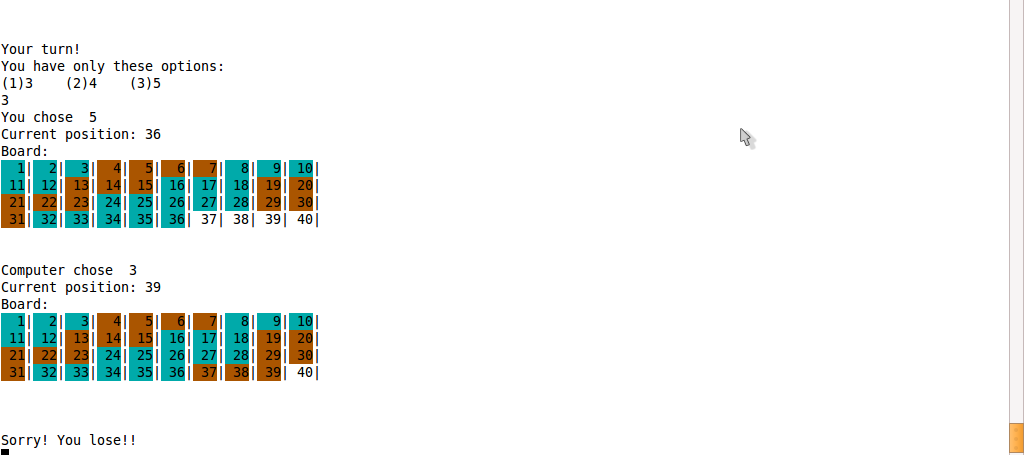
\includegraphics[scale=.30]{l6.png}
\else
%	\includegraphics[scale=0.30]{college logo}
\fi
\end{figure}


\thispagestyle{empty}
\begin{figure}[htb]
\ifpdf
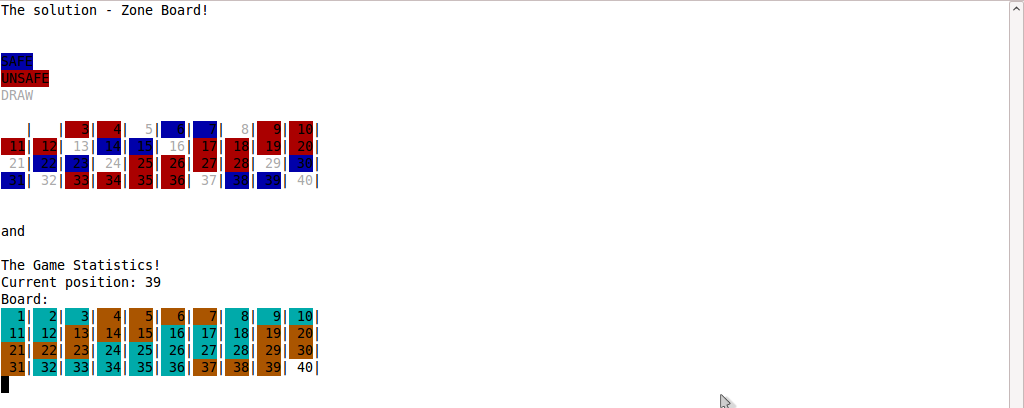
\includegraphics[scale=.40]{l7.png}
\else
%	\includegraphics[scale=0.30]{college logo}
\fi
\end{figure}

\newpage
\thispagestyle{empty}
\begin{figure}[htb]
\ifpdf
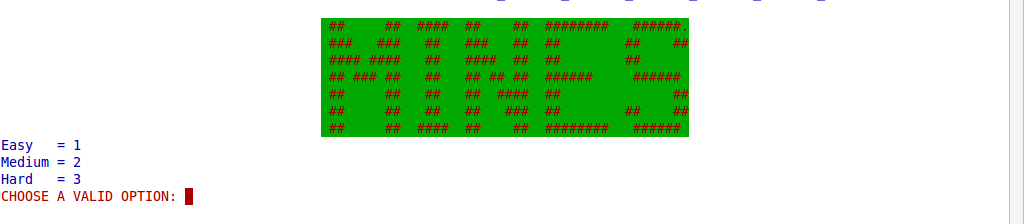
\includegraphics[scale=.20]{m1.png}
\else
%	\includegraphics[scale=0.30]{college logo}
\fi
\end{figure}

\thispagestyle{empty}
\begin{figure}[htb]
\ifpdf
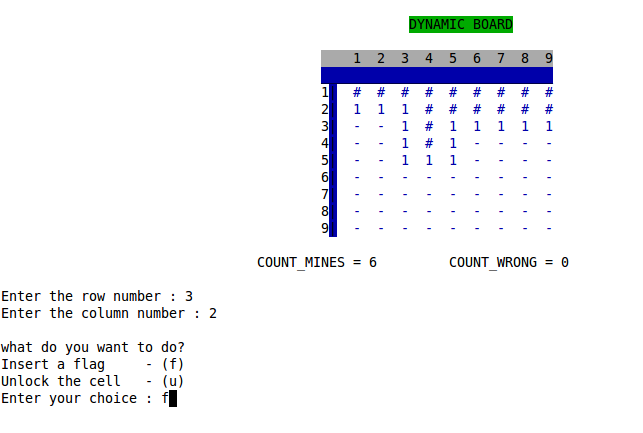
\includegraphics[scale=.40]{m2.png}
\else
%	\includegraphics[scale=0.30]{college logo}
\fi
\end{figure}




\thispagestyle{empty}
\begin{figure}[htb]
\ifpdf
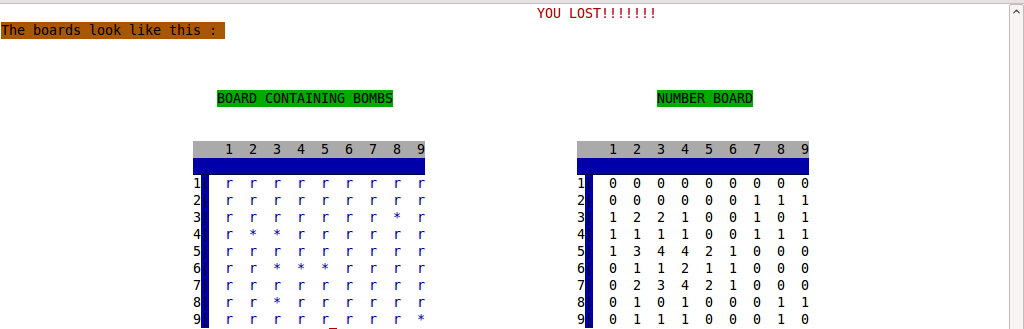
\includegraphics[scale=.40]{m4.png}
\else
%	\includegraphics[scale=0.30]{college logo}
\fi
\end{figure}




\newpage
\section{Results}


Minesweeper:\\

input :unlock the positions in the board by keepin the count of
the mines such that you unlock entire board without clicking any
mines.Here, (.)locked positions,(-)unlocked positions.\\ 
. $|$. $|$. $|$. $|$. $|$. $|$. $|$. $|$. $|$\\
- $|$- $|$. $|$. $|$. $|$1 $|$- $|$. $|$. $|$\\
- $|$1 $|$. $|$. $|$2 $|$- $|$- $|$. $|$. $|$\\ 
- $|$- $|$1 $|$. $|$1 $|$- $|$- $|$. $|$. $|$\\ 
- $|$- $|$2 $|$. $|$1 $|$- $|$. $|$. $|$. $|$\\
- $|$- $|$- $|$. $|$. $|$. $|$. $|$. $|$. $|$\\
. $|$. $|$. $|$. $|$. $|$. $|$. $|$. $|$. $|$\\ 
1 $|$- $|$- $|$- $|$- $|$- $|$. $|$. $|$. $|$\\ 
. $|$. $|$. $|$. $|$. $|$. $|$. $|$. $|$. $|$\\ 

output :If u unlock all positions without selecting any mine,
you WIN.Else you LOSE.\\

Length Conquer Game:\\

input :The total length of the zone say l and three sun-units 
x, y and z.\\
01$|$02$|$03$|$04$|$05$|$06$|$07$|$08$|$09$|$10$|$\\
11$|$12$|$13$|$14$|$15$|$16$|$17$|$18$|$19$|$20$|$\\
21$|$22$|$23$|$24$|$25$|$26$|$27$|$28$|$29$|$30$|$\\
Here l=30,x=3,y=4,z=5.\\

output :if the player does not make it to 30 in his chance 
without any options,he LOSES.\\
Else if he makes it exactly to 30. the game is a DRAW.
If the opponent does not make it to 30 without any draw,
player WINS.\\








\newpage
\section{Conclusion}

A popular technique in Minesweeper is known as "chording". Some of the fastest times ever 
accomplished in Expert level have been said to be achieved with this technique. A strafe
is performed by using the following steps: 1) Flag a cell by pressing, but not releasing,
the right mouse button, 2) drag the mouse, with the right mouse button still pressed, to 
a number that is fully flagged, 3) with the right mouse button still pressed, press and 
release the left mouse button to clear the fully flagged number.
This game is solved basically using brute-force techniques and it does not have any ideal
algorithms,or we can say we can only achieve average efficiency.

Length conquer game is based mainly on greedy' techniques of solving and comes under 
the "zero sum problem".This algorithm we have written has a very good efficiency and 
consumes less time in solving it and also the output can be analysed easily.

This project provided us the exposure to the real life problems related to the above
techniques.We got to know the implementation of these problems in a C as well as c++ 
program.




\end{document}














